\newpage
\section{Case Studies}
\subsection{Multiple Host Headers}

\textbf{Case 1} 讨论当同一个Request中存在多个Host字段时,该如何解析和处理。
\vspace{1ex}

\begin{spacing}{0.8}
	\begin{tcolorbox}
	
		\textbf{RFC 2616}
		Multiple message-header fields with the same \texttt{field-name} {\color{red}{MAY}} be present in a message {\color{red}{ if and only if (隐晦地说明Multiple Host是不允许的)}} the entire \texttt{field-value} for that header field is defined as a comma-separated list. It MUST be possible to combine the multiple header fields into one ``\texttt{field-name: field-value}'' pair, without changing the semantics of the message, by appending each subsequent field-value to the first, each separated by a comma. (Page 22, 4.2, Meassage Headers)
	\end{tcolorbox}
\end{spacing} 

\vspace{1ex}

\begin{spacing}{0.8}
		\begin{tcolorbox}
		\textbf{RFC 7230} 
		A sender {\color{red}{MUST NOT}} generate multiple header fields with the same field name in a message unless either the entire field is defined  as a comma-separated list ...
	
		A recipient MAY combine multiple header fields with the same field name into one ``\texttt{field-name: field-value}'' pair, without changing the semantics of the message, by appending each subsequent field value to the combined field value in order, separated by a comma. (Page 24, 3.2.2, Field Order)
	\end{tcolorbox}
\end{spacing}

\vspace{1ex}

\begin{spacing}{0.8}
	\begin{tcolorbox}
		\textbf{RFC 7230}
		A server {\color{red}{MUST respond with a 400 (Bad Request)}} status code to any HTTP/1.1 request message that lacks a \texttt{Host} header field and to any request message that {\color{red}{contains more than one \texttt{Host} header field}} or a \texttt{Host} header field with an invalid field-value. (Page 44, 5.4,  Host)
	\end{tcolorbox}
\end{spacing}

\vspace{2ex}

\begin{figure*}[!htbp]
	\centering
	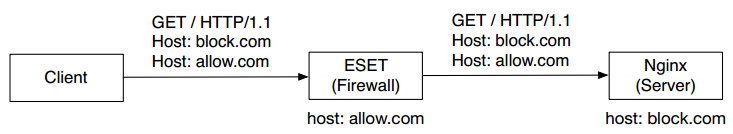
\includegraphics[width=1.0\textwidth]{Preference_Multi-Host.jpg}
	\caption{Preference of multiple \texttt{Host} headers.}
	\label{fig:preference_multi-Host}
\end{figure*}

首先,在同一个Request中出现多个\texttt{Host}本来就是非法的,而ESET和Nginx都允许这种情况出现。其次,面对多个\texttt{Host},二者选择的方式不一样,见下表:

\begin{table}[!htbp]
	\renewcommand\arraystretch{1} 
	\begin{tabular}{|c|c|c|}
		\hline 
		\textbf{Implementation} & \makecell{\textbf{Preference} \\ \textbf{for multiple \texttt{Host}}} & \makecell{\textbf{Request forwarding} \& \\ \textbf{Host interpreting}}  \\  
		\hline 
		ESET & \textbf{Last} \texttt{Host} & 原样转发 \\ 
		\hline 
		Nginx & \textbf{First} \texttt{Host} & \\
		\hline
		\hline
		RFC 2616 & Reject & \\
		\hline
		RFC 7230 & Reject & \makecell{ Absolute-URI中的Host优先\\为Absolute-URI新建一个Host字段\\ Host字段其次} \\
		\hline
	\end{tabular} 
\caption{Case 1}
\end{table}

\textbf{Case 2} 讨论如果Request中同时存在Absolute-URI和Host字段,该如何解析和处理。
\begin{spacing}{0.8}
	\begin{tcolorbox}
		\textbf{RFC 2616}
		An origin server that does differentiate resources based on the host requested MUST use the following rules for determining the requested resource on an HTTP/1.1 request:
		\begin{enumerate}
			\item If \texttt{Request-URI} is an \texttt{absoluteURI}, the host is part of the \texttt{Request-URI}. Any \texttt{Host} header field value in the request MUST be ignored.
			\item If the \texttt{Request-URI} is not an \texttt{absoluteURI}, and the request includes a \texttt{Host} header field, the host is determined by the \texttt{Host} header field value.
			\item If the host as determined by rule 1 or 2 is not a valid host on the server, the response MUST be a 400 (Bad Request) error message. (Page 25, 5.2, The Resource Identified by a Request)
		\end{enumerate}
	\end{tcolorbox}
\end{spacing}
\vspace{1ex}
\begin{spacing}{0.8}
	\begin{tcolorbox}
		\textbf{RFC 7230 有关如何解析Host和转发Request}
		
		When a proxy receives a request with an absolute-form of request-target, the proxy MUST ignore the received \texttt{Host} header field (if any) and instead replace it with the host information of the
		request-target (Absolute-URI中的Host信息优先). A proxy that forwards such a request {\color{red}{MUST generate a new Host field-value based on the received request-target}} rather than forward the received \texttt{Host} field-value. (Page 44, 5.4, Host)
	\end{tcolorbox}
\end{spacing}

总结起来就是说:如果有\texttt{Absolute-URI},则取这里面的Host,\texttt{Host}字段中的值被忽略。如果没有\texttt{Absolute-URI},则以\texttt{Host}字段的值为准。否则,报错400 Bad Request。

\begin{figure*}[!htbp]
	\centering
	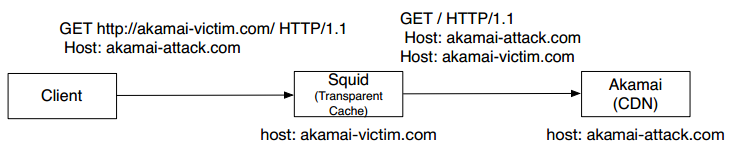
\includegraphics[width=1.0\linewidth]{images/AbsoluteURI_Host}
	\caption{Absolute URI with \texttt{Host} headers.}
	\label{fig:absolute-uri_host}
\end{figure*}

\begin{table}[!htbp]
	\renewcommand\arraystretch{1}
	\centering
	\begin{tabular}{|l|c|c|c|l|c|}
		\hline
		\multicolumn{2}{|c}{\multirow{3}{*}{\tabincell{l}{Implementation\\/Specification}}} & 
		\multicolumn{2}{|c|}{\multirow{2}{*}{\tabincell{l}{Prefer Absolute-URI\\vs. Prefer Host header}}} &
		\multicolumn{1}{c|}{\multirow{3}{*}{Request forwarding}} &
		\multicolumn{1}{c|}{\multirow{3}{*}{\tabincell{c}{Preference\\for multiple\\Host}}}
		\\ 
		\multicolumn{2}{|l|}{} & \multicolumn{2}{c|}{} & &
		\\ \cline{3-4}
		\multicolumn{2}{|l|}{} & \textbf{Preference} & \textbf{Consistency} & &
		\\ \hline
		Squid & \tabincell{c}{Transparent\\Cache} & Absolute-URI & Optional & {\tabincell{l}{1.Generate a new \\ Host header \\for Absolute-URI \\and select this one. \\ 2.Forward\\ space-preceded \\Host headers as-is}} & Prefer first
		\\ \hline
		Akamai & CDN & Host header & Optional & & Prefer first
		\\ \hline
		\hline
		\multicolumn{1}{|c|}{\multirow{2}{*}{Specification}}  & RFC 2616 & Absolute-URI & Not Specified & & Reject
		\\ \cline{2-6}
		& RFC 7230 & Absolute-URI & Must & & Reject
		\\ \hline
	\end{tabular}
\caption{Case 2}
\end{table}

\pagebreak
\textbf{Case 3} 讨论多Host header,同时伴随前置空格(preceding space)的情况。
\begin{spacing}{0.8}
	\begin{tcolorbox}
		\textbf{RFC 7230}
		A field value {\color{red}{might}} be preceded and/or followed by optional whitespace (OWS); a single SP preceding the field-value is preferred for consistent readability by humans. The field value does not include any leading or trailing whitespace: OWS occurring before the first non-whitespace octet of the field value or after the last non-whitespace octet of the field value ought to be excluded by parsers when extracting the field value from a header field. (Page 25, 3.2.4, Field Parsing) {\color{red}{隐约地说明field value最前头或最后头有空格是允许的!}}
	\end{tcolorbox}
\end{spacing}

\begin{figure}[!htbp]
	\centering
	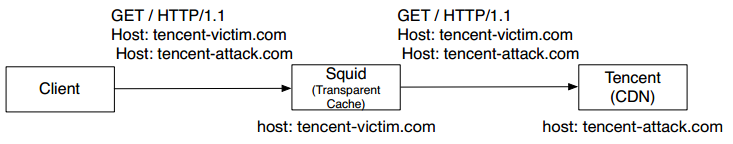
\includegraphics[width=1.0\linewidth]{images/Multi-Host_Preceding_Space}
	\caption{Multiple \texttt{Host} headers with preceding space.}
	\label{fig:multi-host_precedingspace}
\end{figure}
 
\begin{table}[!htbp]
	\renewcommand\arraystretch{1}
	\begin{tabular}{|c|c|c|c|c|}
		\hline
		\multicolumn{2}{|c|}{\multirow{2}{*}{\tabincell{l}{Implementation\\/Specification}}} & 
	\multirow{2}{*}{\tabincell{c}{Space-preceded Host\\ as first Host header}} &
	\multirow{2}{*}{\tabincell{c}{Other Space-preceded\\Host header}} &
	\multirow{2}{*}{\tabincell{c}{Space-succeeded\\Host header}} 
	\\ 
	\multicolumn{2}{|c|}{} & \multirow{2}{*}{} & \multirow{2}{*}{}& \multirow{2}{*}{}
	\\ \hline
	Squid & \tabincell{c}{Transparent\\Cache} & \tabincell{l}{If no Host header \\ before:recognize \\ Else: {\color{red}{not recognize}}} & \tabincell{l}{If no Host header\\before:recognize\\Else: not recognize} & \tabincell{l}{If no Host header\\before:recognize\\Else: not recognize}
	\\ \hline
	Tencent & CDN & Recognize & Recognize & Recognize 
	\\ \hline \hline 
	\multirow{2}{*}{Specification}  & RFC 2616 & Reject & Line folding & Recognize 
	\\ \cline{2-5}
	& RFC 7230 & Recognize & Recognize & Recognize 
	\\ \hline
\end{tabular}
\caption{Case 3-1, {\color{red}{Recognize: accepting as valid host field}},{\color{red}{Reject: 400 Bad Requests}}, {\color{red}{Reject: Not recognize:either ignoring or accepting as an unknown header field}}.}
\end{table}

\begin{table}[!htbp]
	\renewcommand\arraystretch{1}
	\centering
	\begin{tabular}{|c|c|c|}
		\hline
		\multicolumn{2}{|c|}{\multirow{2}{*}{Implementation/Specification}} &
		\multirow{2}{*}{Preference for multiple Host}
		\\ 
		\multicolumn{2}{|c|}{} & 
		\\ \hline
		Squid & Transparent Cache & Prefer first 
		\\ \hline
		Tencent & CDN & Prefer last
		\\ \hline \hline
		\multirow{2}{*}{Specification} & RFC 2616 & Reject
		\\ \cline{2-3}
		& RFC 7230 & Reject
		\\ \hline
	\end{tabular}
\caption{Case 3-2}
\end{table}


Case 4: 讨论RFC Ambiguities可能出现的地方
\begin{spacing}{0.8}
	\begin{tcolorbox}
		\textbf{RFC 7230} A field value might be preceded and/or followed by optional whitespace (OWS) ...
	\end{tcolorbox}
\end{spacing}

\vspace{1ex}

\begin{spacing}{0.8}
	\begin{tcolorbox}
		A server that receives an obs-fold in a request message MUST {\color{red}{either}} reject the message by
		sending a 400 (Bad Request) ... {\color{red}{or}} replace each received obs-fold with one or more SP octets prior to interpreting the field value {\color{red}{or}} forwarding the message downstream.
		
		A proxy or gateway MUST {\color{red}{either}} discard the message and replace it with a 502 (Bad Gateway) response {\color{red}{or}} replace each received obs-fold with one {\color{red}{or}} more SP octets prior to interpreting the field value or forwarding the message downstream.  (Page 25-26, 3.2.4, Field Parsing)
	\end{tcolorbox}
\end{spacing}

\vspace{1ex}

\begin{spacing}{0.8}
	\begin{tcolorbox}
	A proxy or gateway MUST {\color{red}{either}} discard the message and replace it with a 502 (Bad Gateway) response {\color{red}{or}} replace each received obs-fold with one {\color{red}{or}} more SP octets prior to interpreting the field value or forwarding the message downstream.  (Page 26, 3.2.4, Field Parsing)
	\end{tcolorbox}
\end{spacing}